\chapter{Ensemble}
\section{Introduction}
就是好几个模型一起上,在分类或是回归问题上能够得到一个更好的结果。

\section{Framework of Ensemble}
假设你在做一个分类任务,首先你要有一大堆不同的的classifiers,它们要一起完成
一个分类任务,就好像是玩游戏时各自的分工是不一样的,我们需要找到一个方法替这些
classifiers找到一个好的分工从而提高分类的准确率。

\section{Ensemble: Bagging}
注意: Bagging适用于很复杂的模型
\subsection{Review: Bias v.s. Variance}
如果是很简单的模型就会有很小的Variance和很大的Bias,如果模型很复杂就会有很
大的Varience和很小的Bias。我们将这些很复杂的模型平均起来就可以的减小Variance
从而提高系统的性能。
\subsection{Bagging}
怎么做Bagging呢,假设我们有N笔Training example每次从中随机抽取$N^`$个examples
来训练一个模型。如下图一共抽取了四次训练了四个不同模型。
\begin{figure}[H]
    \centerline{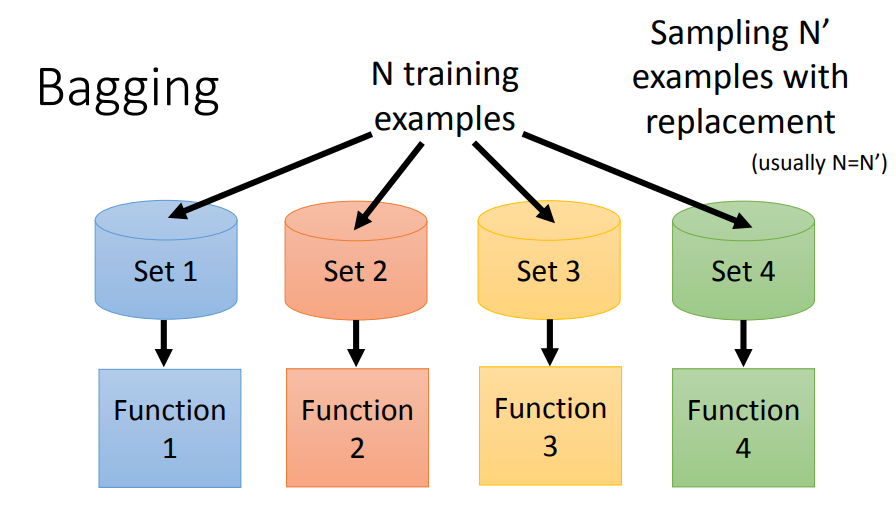
\includegraphics[scale=0.3]{Part1/Chapter/images/bagging1.png}}
    \caption{Training Bagging}
\end{figure}

Bagging适用于很复杂很容易过拟合的模型。在测试阶段如果是回归问题那么就求这四个输出
的平均值作为结果,如果是分类问题那么我们使用voting(选择出现次数最多的那个类最为最终输出)。
\begin{figure}[H]
    \centerline{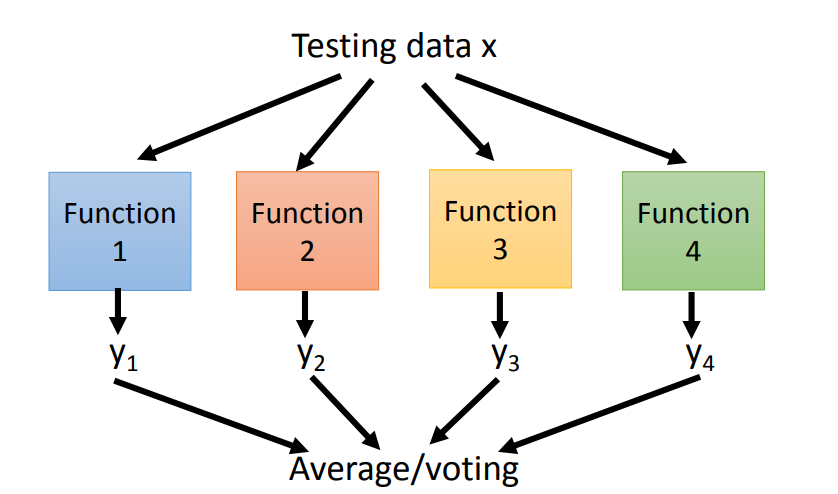
\includegraphics[scale=0.3]{Part1/Chapter/images/bagging2.png}}
    \caption{Training Bagging}
\end{figure}

\subsection{Decision Tree}
决策树非常容易过拟合,只要树够深就能100\%拟合训练集,这里是做了一个实验让决策树
判断像素点是不是属于初音。
\begin{figure}[H]
    \centerline{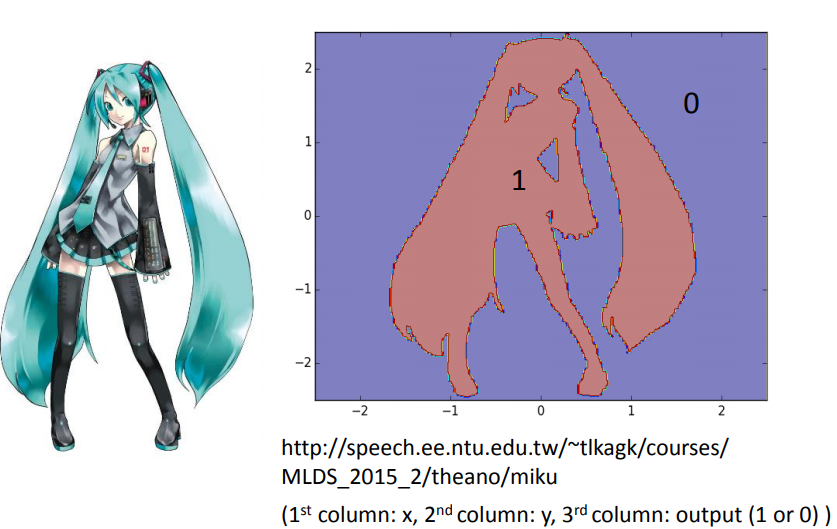
\includegraphics[scale=0.3]{Part1/Chapter/images/experiment-miku.png}}
    \caption{Experiment: Function of Miku}
\end{figure}

下图是我们使用单个决策树的情况,可以看出来当输的深度达到20时决策树就可以完美的拟合啦
\begin{figure}[H]
    \centerline{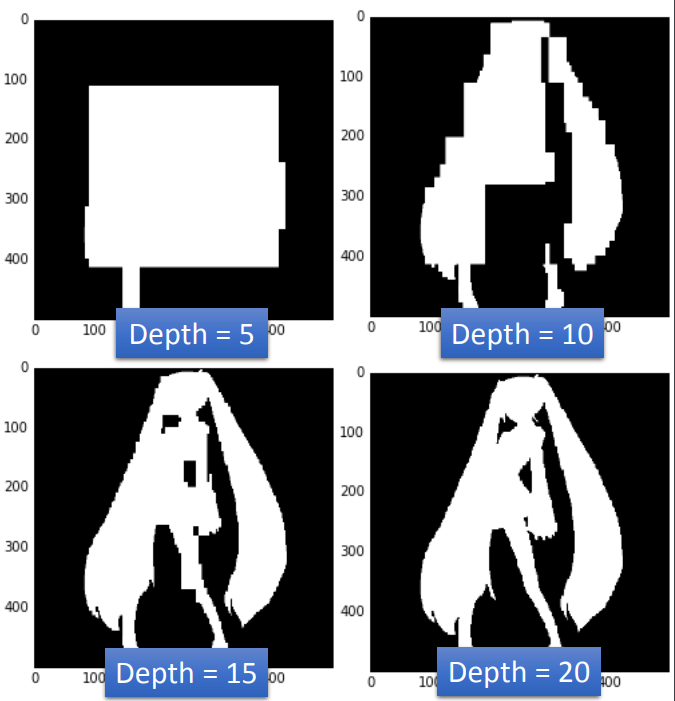
\includegraphics[scale=0.3]{Part1/Chapter/images/experiment.png}}
    \caption{Experiment: Function of Miku(Decision Tree)}
\end{figure}

\subsection{Random Forest}

Random Forest 就是 Bagging of decision tree, 随机森林在对每棵树随机抽取数据
训练外还限制了一些features这个就需要具体看一下随机森林的算法了。用Out-of-bag(OOB)
对Bagging算法进行验证。

给出数据分配图一共4笔数据,有四个决策树,每个决策树只能看到两笔数据那么就可以拿
另外两笔数据来验证模型的效果,如图3.6。
\begin{figure}[H]
    \centerline{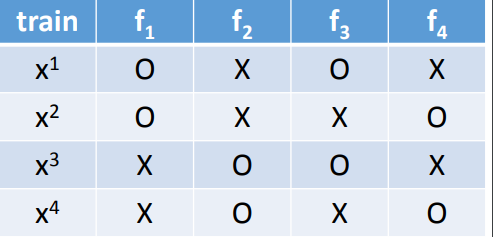
\includegraphics[scale=0.3]{Part1/Chapter/images/oob1.png}}
    \caption{数据分配}
\end{figure}

如$f_2$没看过$x^1$, $f_4$也没看$x^1$,那么就可以用$x^1$验证$f_2$和$f_4$  Bagging后的效果。
\begin{figure}[H]
    \centerline{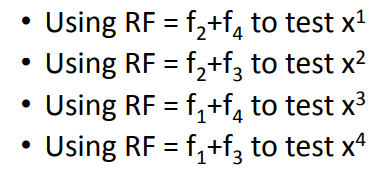
\includegraphics[scale=0.3]{Part1/Chapter/images/oob2.png}}
    \caption{Out-of-bag}
\end{figure}

决策树得到的结果比单个决策树要平滑一些。
\begin{figure}[H]
    \centerline{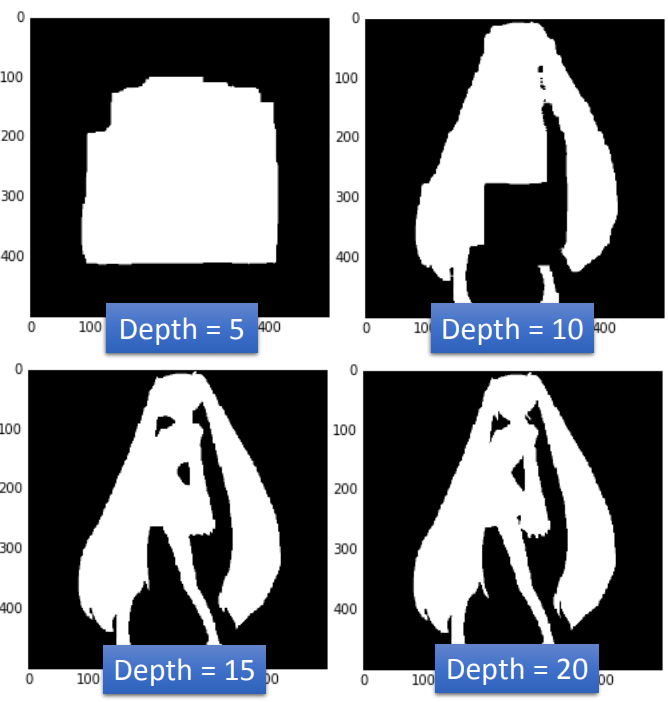
\includegraphics[scale=0.3]{Part1/Chapter/images/experiment2.png}}
    \caption{Experiment: Function of Miku(Random Forest)}
\end{figure}

\section{Ensemble: Boosting}
注意:Boosting是用于弱分类器

\subsection{Boosting}
使用Boosting有一个很强的保证只要你有一个正确率大于50\%的分类器,经过Boosting之后
你会得到一个错误率是0\%的分类器。

\subsection{Framework of boosting}
首先你要有一个分类器$f_1(x)$,然后找到另一个分类器$f_2(x)$来帮助$f_1(x)$
,但是$f_2(x)$和$f_1(x)$是互补的,$f_2(x)$要做$f_1(x)$做不到的事情,如果二者特别相似帮助也不会很大,
得到$f_2(x)$之后再用$f_3(x)$来帮助$f_2(x)$......重复下去。
(Boosting训练是有顺序的)
\\
假设我们有一个数据集{{${(x^1, \hat{y}^1), (x^2, \hat{y}^2), ..., (x^n, \hat{y}^n)}$}} 
其中$\hat{y}^i = \textpm 1$是一个二分类问题,那么我们该怎么得到不同的分类器呢?\\
我们可以用不同的数据来训练分类器, 有两种方法来生成不同的数据。

\begin{itemize}
    \item 1. 随机从训练集中抽取数据进行训练
    \item 2. 给训练集一个权重
\end{itemize}


随机抽取数据不必多说,给数据权重就是每一笔数据给一个$u^i$作为权重然后我们的数据集就成了{{${(x^1, \hat{y}^1,u^1), (x^2, \hat{y}^2, u^2), ..., (x^n, \hat{y}^n, u^n)}$}}
然后 我们要改变我们的Loss Function:$L(f) = \sum_{i=0}^{n}u^il(f(x^i), \hat{y}^i)$,这样如果某笔data的权重很大造成loss很大,就会受到更多的关注。
(初始权重为1)
\subsection{Idea of Adaboost}
Adaboost的思想就是先训练$f_1(x)$(准确度必然大于50\%), 然后更改权重$u$,使$f_1(x)$在新的数据上得到准确度等于50\%, 再用这个数据训练$f_2(x)$
这样就让$f_2(x)$和$f_1(x)$互补啦,因为二者学习的是不同的数据。给出更改权重的公式:\\\\
\centerline{${\epsilon}_1$ 是$f_1(x)$的错误率}\\\\

\begin{equation*}
    Z_1 = \sum_{i=1}^n u_1^i
\end{equation*}

\begin{equation*}
    {\epsilon}_1 = \frac{\sum_{i=0}^{n} u_1^i \delta(f(x^i) \neq \hat{y}^i)}{Z_1}, {\epsilon}_1 < 0.5
\end{equation*}
其中 $\delta(f(x^i) \neq \hat{y}^i) = 0$,如果$f(x^i) \neq \hat{y}^i$
,$\delta(f(x^i) \neq \hat{y}^i) = 1$,如果$f(x^i) = \hat{y}^i$\\\\
要找到一个$u_2$替换掉上面的$u_1$使
\begin{equation*}
    \frac{\sum_{i=0}^{n} u_2^i \delta(f(x^i) \neq \hat{y}^i)}{Z_2} = 0.5
\end{equation*}
\\

下面给一个re-weighting的例子, $\epsilon_1 = 0.25$, 然后我们将分类正确的权重除以$\sqrt{3}$降低影响,
 将分类错误的权重乘以$\sqrt{3}$增大影响(至于为什么是$\sqrt{3}$下面会给出详细的解答)。然后 $\frac{\sum_{i=0}^{n} u_2^i \delta(f(x^i) \neq \hat{y}^i)}{Z_2} = 0.5$
 再重新训练一个$f_2(x)$使$\epsilon_2 < 0.5$。

\begin{figure}[H]
    \centerline{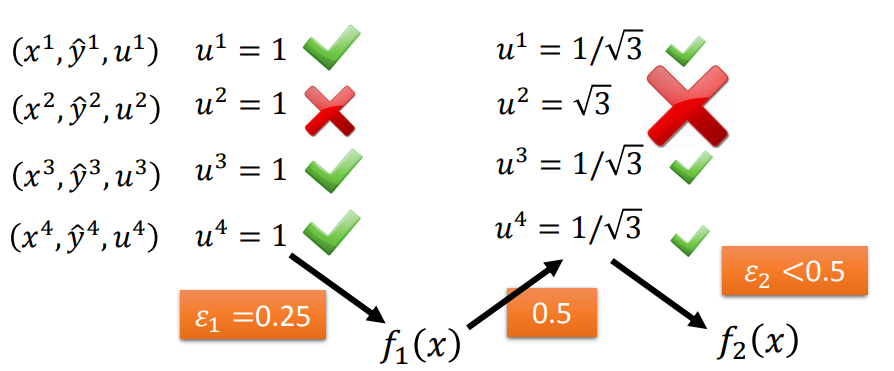
\includegraphics[scale=0.3]{Part1/Chapter/images/reweightexample1.png}}
    \caption{Re-weighting example}
\end{figure}

如果一个数据被分类正确那么就把它的权重除以一个数$d_1$($d_1$ > 1),如果分类错误就把对应权重乘以$d_1$($d_1$ > 1), 那么怎么求$d_1$,下面给出推倒。

\begin{equation*}
    Z_1 = \sum_{i=1}^m u_1^i
\end{equation*}

\begin{equation*}
    {\epsilon}_1 = \frac{\sum_{i=0}^{n} u_1^i \delta(f(x^i) \neq \hat{y}^i)}{Z_1}, {\epsilon}_1 < 0.5
\end{equation*}

\begin{equation*}
    \frac{\sum_{i=0}^{n} u_2^i \delta(f(x^i) \neq \hat{y}^i)}{Z_2} = 0.5
\end{equation*}
\\

\begin{equation*}
    \sum_{i=0}^{n} u_2^i \delta(f(x^i) \neq \hat{y}^i) = \sum_{f(x_i) \neq \hat{y}_i {i=1}}^n u_1^i d_1
\end{equation*}

\begin{equation*}
    Z_2 = \sum_{f(x_i) \neq \hat{y}_i {i=1}}^n u_2^i + \sum_{f(x_i) = \hat{y}_i {i=1}}^n u_2^i
\end{equation*}

\begin{equation*}
    Z_2 = \sum_{f(x_i) \neq \hat{y}_i {i=1}}^n u_1^i d_1 + \sum_{f(x_i) = \hat{y}_i {i=1}}^n \frac{u_1^i}{d_1}
\end{equation*}

将方程代入原式

\begin{equation*}
    \frac{ \sum_{f(x_i) \neq \hat{y}_i {i=1}}^n u_1^i d_1}{\sum_{f(x_i) \neq \hat{y}_i {i=1}}^n u_1^i d_1 + \sum_{f(x_i) = \hat{y}_i {i=1}}^n \frac{u_1^i}{d_1}}
    = 0.5
\end{equation*}


将上面的式子化简得到
\begin{equation*}
    \sum_{f(x_i) \neq \hat{y}_i {i=1}}^n u_1^i d_1 = \sum_{f(x_i) = \hat{y}_i {i=1}}^n \frac{u_1^i}{d_1}
\end{equation*}
将$d_1$拿出来得到
\begin{equation*}
    d_1\sum_{f(x_i) \neq \hat{y}_i {i=1}}^n u_1^i  =  \frac{1}{d_1}\sum_{f(x_i) = \hat{y}_i {i=1}}^n u_1^i
\end{equation*}

\begin{equation*}
    \frac{\sum_{f(x_i) \neq \hat{y}_i {i=1}}^n u_1^i}{Z_1} = \epsilon_1 >>> \sum_{f(x_i) \neq \hat{y}_i {i=1}}^n u_1^i = Z_1 \epsilon_1
\end{equation*}

\begin{equation*}
    \frac{\sum_{f(x_i) = \hat{y}_i {i=1}}^n u_1^i}{Z_1} = 1 - \epsilon_1 >>> \sum_{f(x_i) = \hat{y}_i {i=1}}^n u_1^i = Z_1 (1 - \epsilon_1)
\end{equation*}

将上述结果带入到$d_1\sum_{f(x_i) \neq \hat{y}_i {i=1}}^n u_1^i  =  \frac{1}{d_1}\sum_{f(x_i) = \hat{y}_i {i=1}}^n u_1^i$ 得到
$d_1 = \sqrt{\frac{(1 - \epsilon_1)}{\epsilon_1}} > 1$ 

\subsection{Algorithm for AdaBoost}
由$d_t$换成$\alpha_t$ 简化了式子, 最终括号一应该填$-y_tf_t(x)$
\begin{figure}[H]
    \centerline{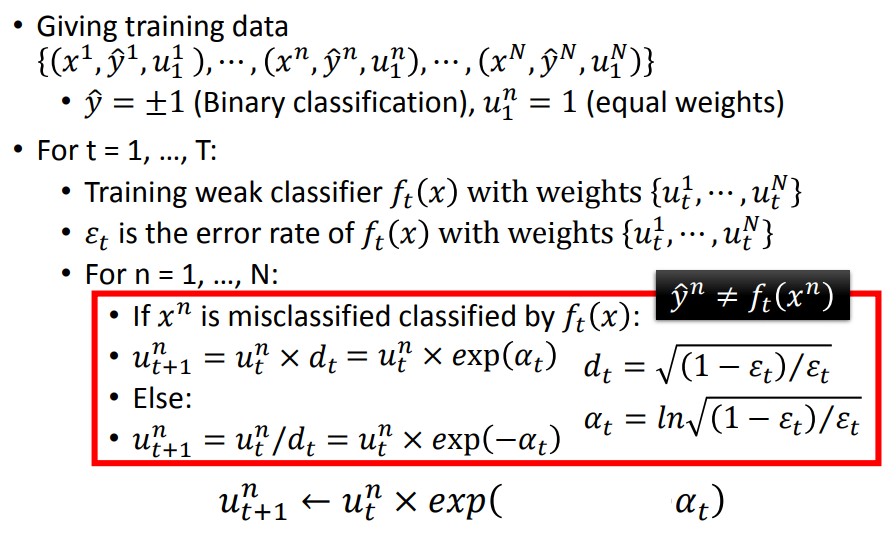
\includegraphics[scale=0.3]{Part1/Chapter/images/algorithmforadaboost1.png}}
    \caption{Algorithm for AdaBoost 1}
\end{figure}

在算最终结果时也要乘上$\alpha_t$,这样做能让$\epsilon$高的分类器得到更高的分数
\begin{figure}[H]
    \centerline{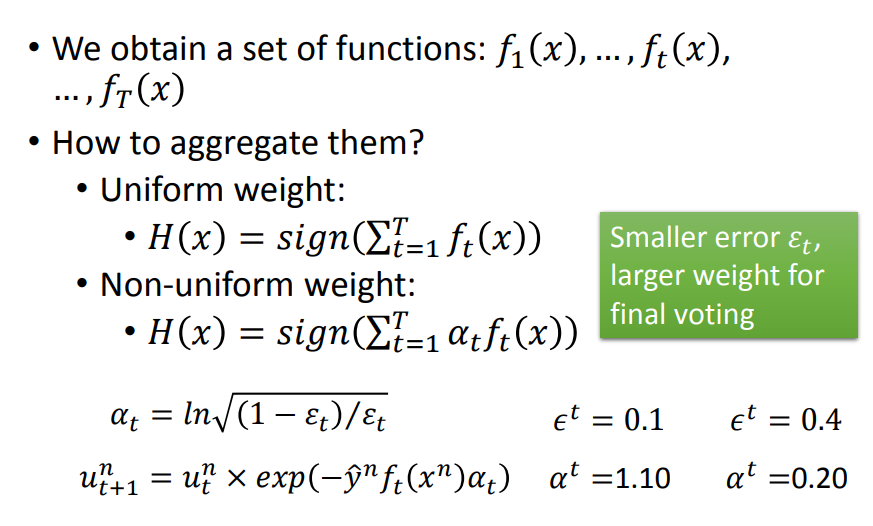
\includegraphics[scale=0.3]{Part1/Chapter/images/afa2.png}}
    \caption{Algorithm for AdaBoost 2}
\end{figure}
\subsection{Toy Example}

用3个weak classifier = decision stump 随便切一刀
\begin{itemize}
    \item Step 1:
    \\
    \begin{figure}[H]
        \centerline{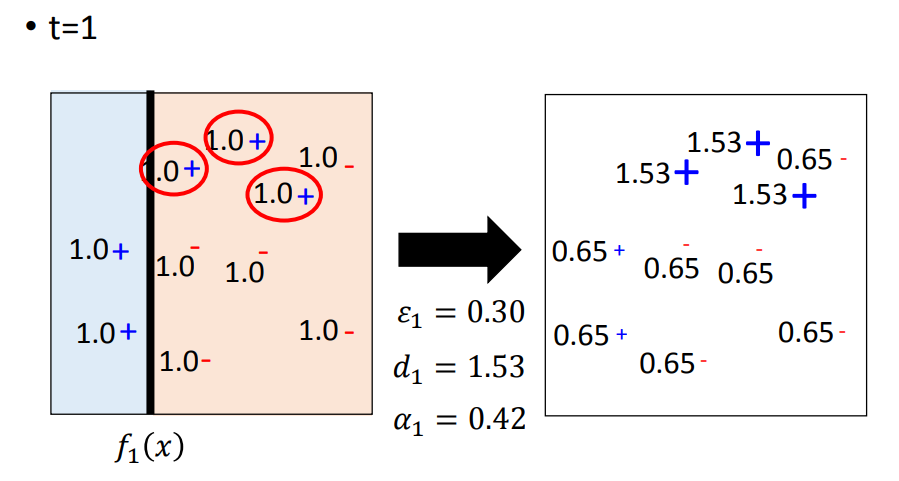
\includegraphics[scale=0.3]{Part1/Chapter/images/toyexample1.png}}
        \caption{Toy Example Step 1}
    \end{figure}
    \item Step 2:
    \\
    \begin{figure}[H]
        \centerline{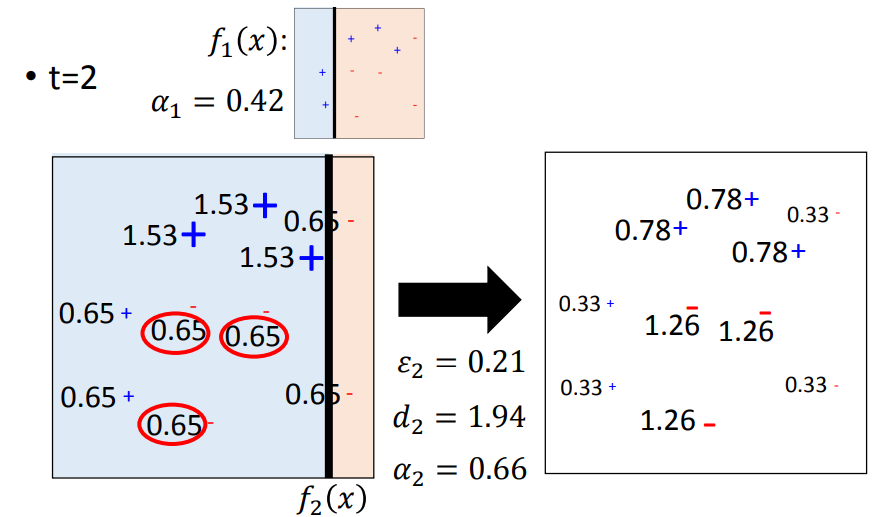
\includegraphics[scale=0.3]{Part1/Chapter/images/toyexample2.png}}
        \caption{Toy Example Step 2}
    \end{figure}
    \item Step 3:
    \\
    \begin{figure}[H]
        \centerline{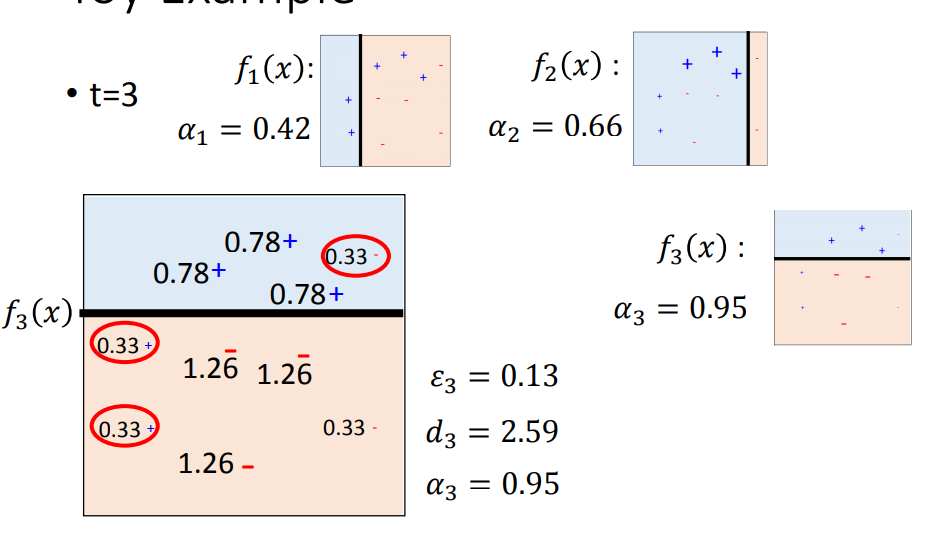
\includegraphics[scale=0.3]{Part1/Chapter/images/toyexample3.png}}
        \caption{Toy Example Step 3}
    \end{figure}
    \item Step 4:
    \\
    \begin{figure}[H]
        \centerline{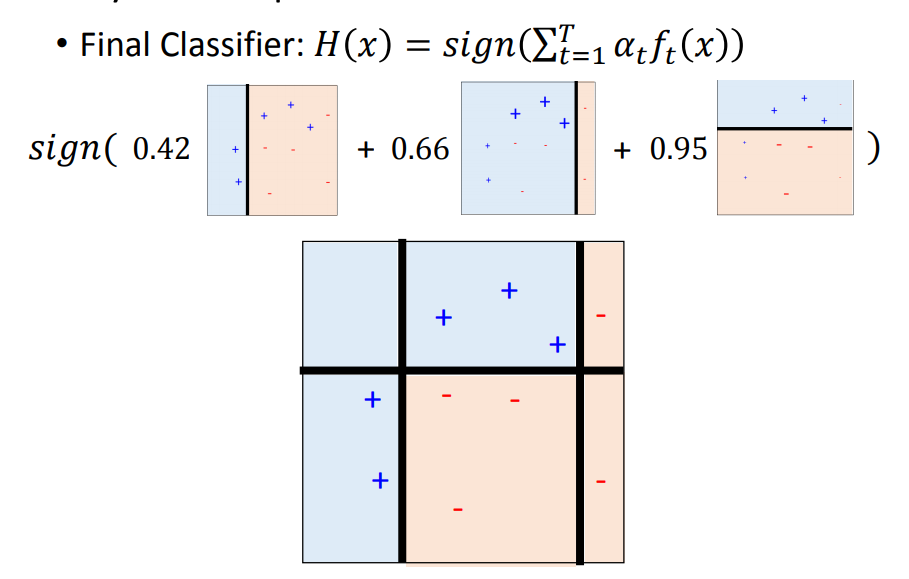
\includegraphics[scale=0.3]{Part1/Chapter/images/toyexample4.png}}
        \caption{Toy Example Step 4}
    \end{figure}
\end{itemize}

\subsection{More Detial in Adaboost}

最终的分类$H(x)$的方程是:
\begin{equation*}
    H(x) = sign(\sum_{t=1}^T \alpha_t f_t(x))
\end{equation*}

\begin{equation*}
    g(x) = \sum_{t=1}^T \alpha_t f_t(x)
\end{equation*}
训练数据上的错误率为(有N笔数据):

\begin{equation*}
    Error Rate = \frac{1}{N} \sum_{n=1}^N \delta(H(x^n) \neq \hat{y}^n)
    = \frac{1}{N} \sum_{n=1}^N \delta(\hat{y}^n g(x^n) < 0)
\end{equation*}

ErrorRate存在一个上限:


\begin{equation*}
    Error Rate \leq \frac{1}{N} \sum_{n=1}^N  \exp(-\hat{y}^n g(x^n))
\end{equation*}


图中绿线代表$\delta(\hat{y}^n g(x^n) < 0)$
蓝线代表$\exp(-\hat{y}^n g(x^n))$, 横坐标是$\hat{y}^n g(x^n)$

\begin{figure}[H]
    \centerline{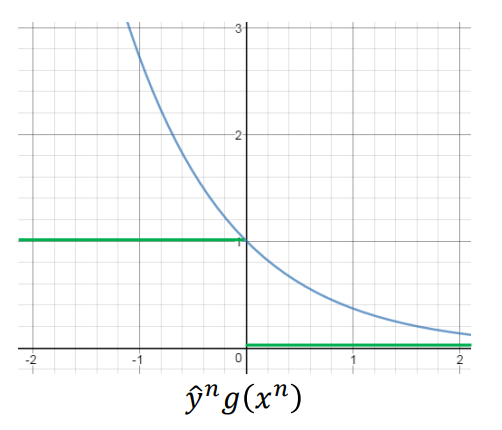
\includegraphics[scale=0.5]{Part1/Chapter/images/upperband.png}}
    \caption{上限}
\end{figure}

我们要证明上限越来越小

\begin{equation*}
    Z_t = \sum_{i=1}^n u_t^i
\end{equation*}
\begin{equation*}
    Z_{t+1} = \sum_{i=1}^n u_{t+1}^i
\end{equation*}

\begin{figure}[H]
    \centerline{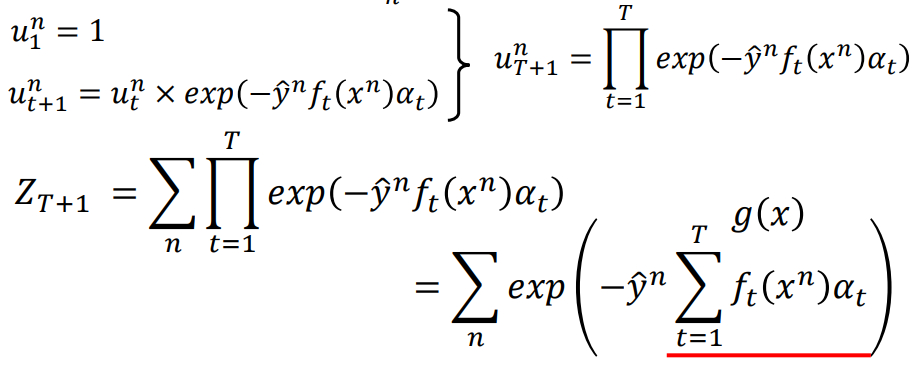
\includegraphics[scale=0.3]{Part1/Chapter/images/zt+1.png}}
\end{figure}

看懂上面的推导之后我们发现$\frac{1}{N} Z_{t+1} = \frac{1}{N} \sum_{n=1}^N  \exp(-\hat{y}^n g(x^n))$
所以能证明$Z$越来越小就ok了。

\begin{figure}[H]
    \centerline{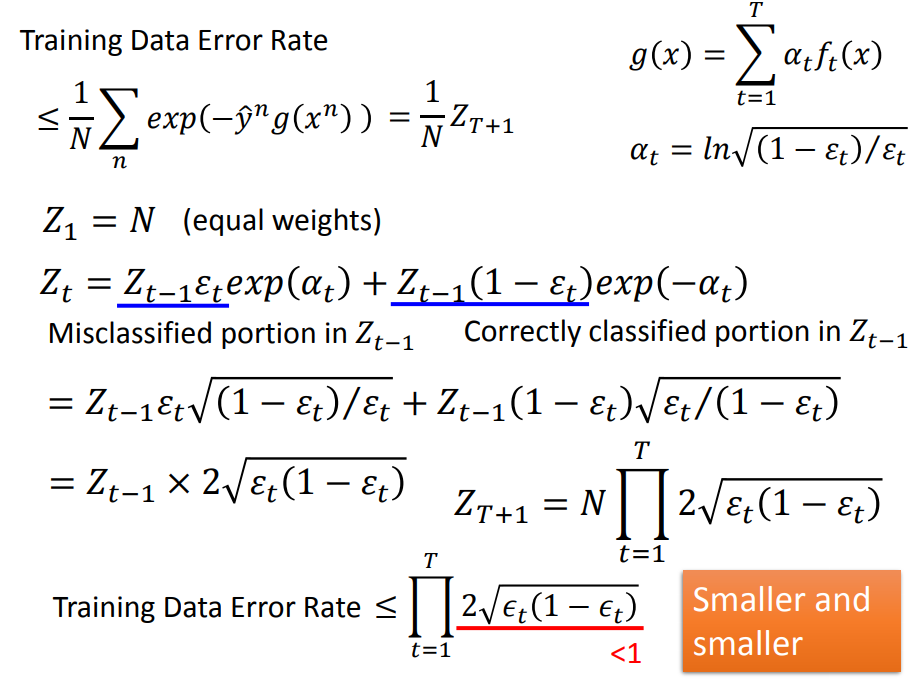
\includegraphics[scale=0.5]{Part1/Chapter/images/proofzt.png}}
    \caption{证明$Z_t$越来越小}
\end{figure}

Adaboost有很神奇的现象,当在training上的error达到零时,在test上的error还可以下降原因是权重可以增加$Margin$
其实原理很简单, AdaBoost的error会无限接近于零但不是零。
\begin{figure}[H]
    \centerline{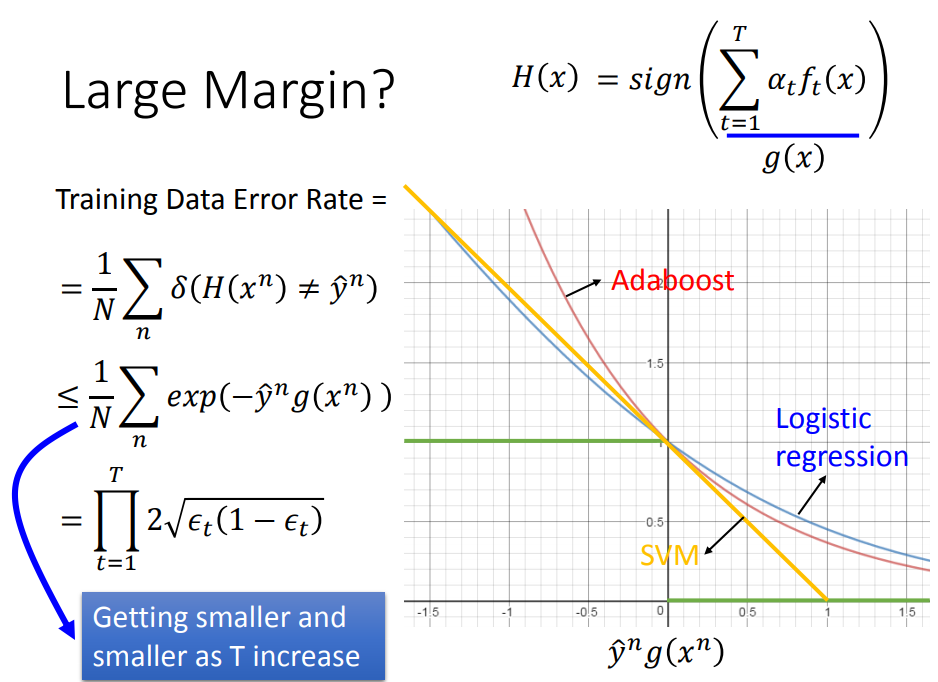
\includegraphics[scale=0.5]{Part1/Chapter/images/largemargin.png}}
    \caption{证明Test上的error rate会变小}
\end{figure}
我们用深度是5的决策树进行Adaboost效果要比在单棵树上好太多。

\begin{figure}[H]
    \centerline{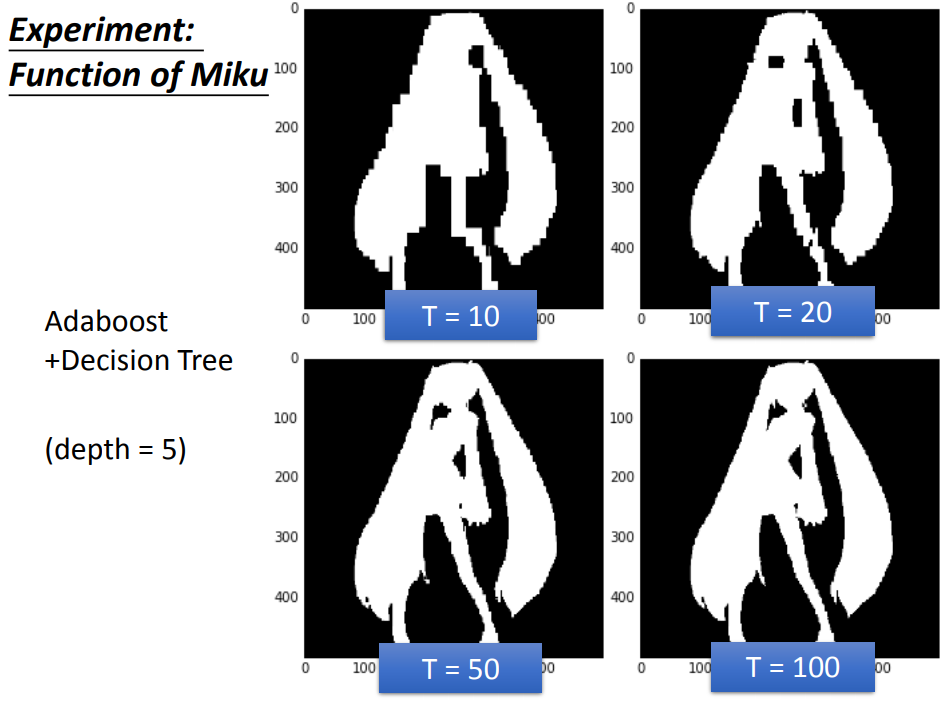
\includegraphics[scale=0.5]{Part1/Chapter/images/adaboostexp.png}}
    \caption{AdaBoost Experienment}
\end{figure}
\subsection{Gradient Boosting}
使用梯度下降的角度来阐释Boosting, 只不过使我们的梯度和LearningRate可以直接求出来,我们可以修改Boosting的object function来达到不同目的。
\begin{figure}[H]
    \centerline{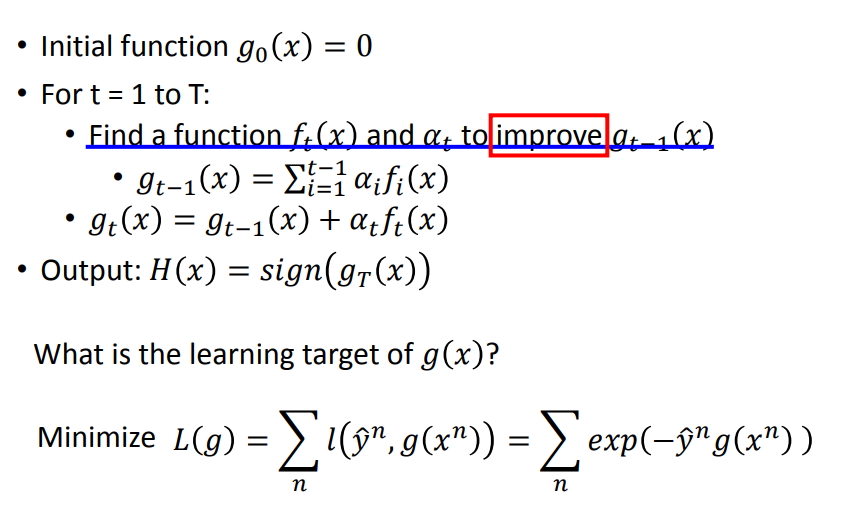
\includegraphics[scale=0.5]{Part1/Chapter/images/gb1.png}}
\end{figure}
\begin{figure}[H]
    \centerline{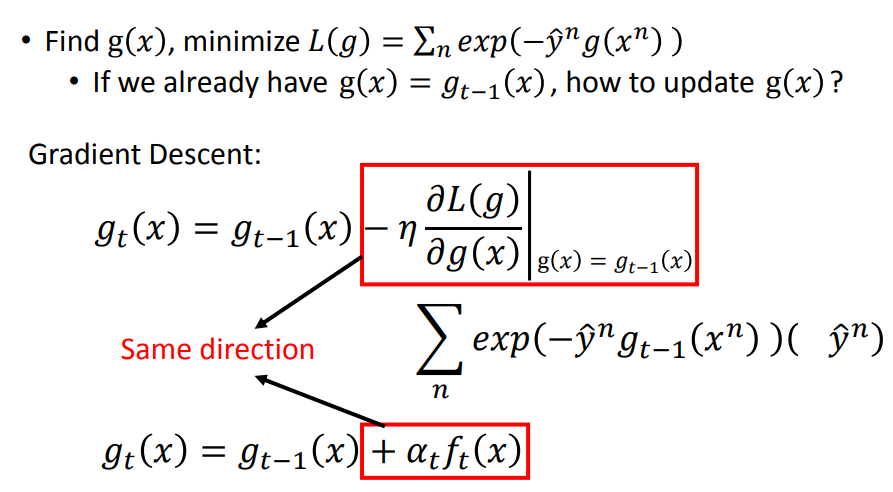
\includegraphics[scale=0.5]{Part1/Chapter/images/gb2.png}}
   
\end{figure}
\begin{figure}[H]
    \centerline{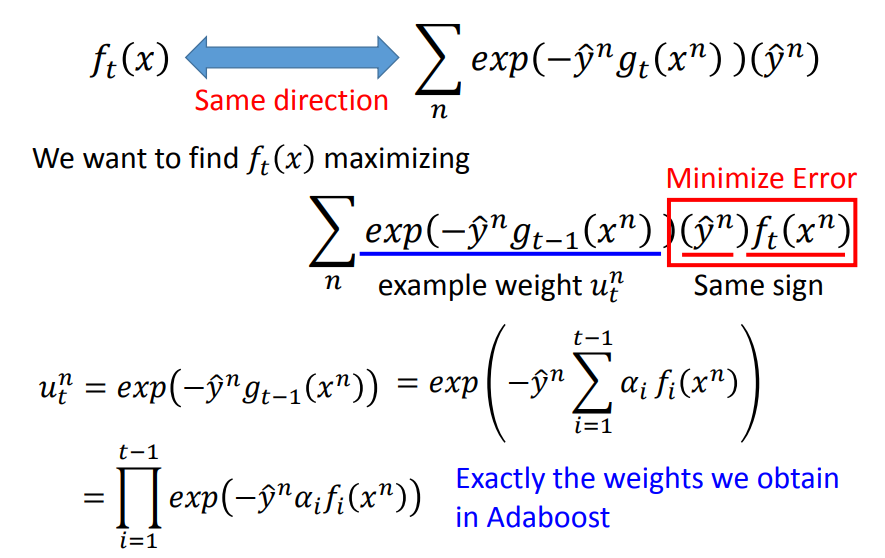
\includegraphics[scale=0.5]{Part1/Chapter/images/gb3.png}}
\end{figure}
\begin{figure}[H]
    \centerline{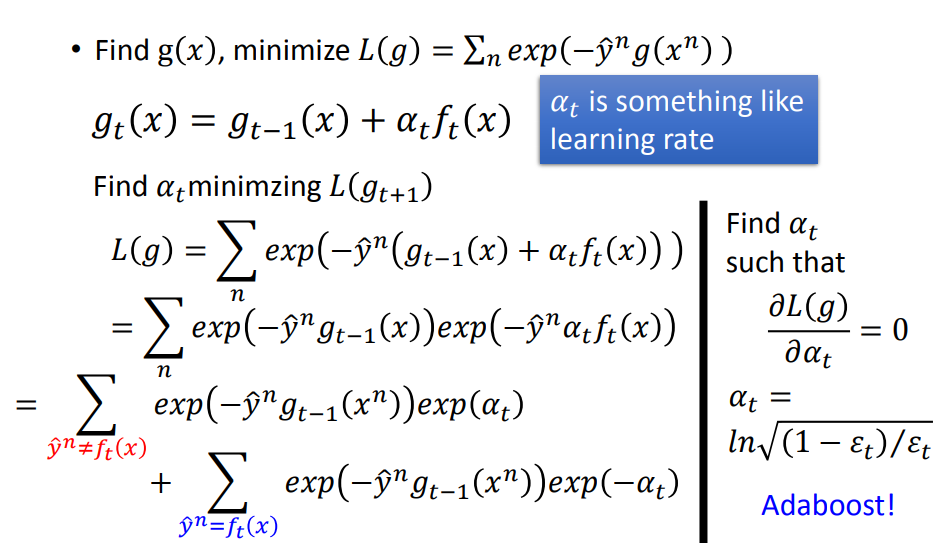
\includegraphics[scale=0.5]{Part1/Chapter/images/gb4.png}}
\end{figure}


\section{Voting}
\begin{figure}[H]
    \centerline{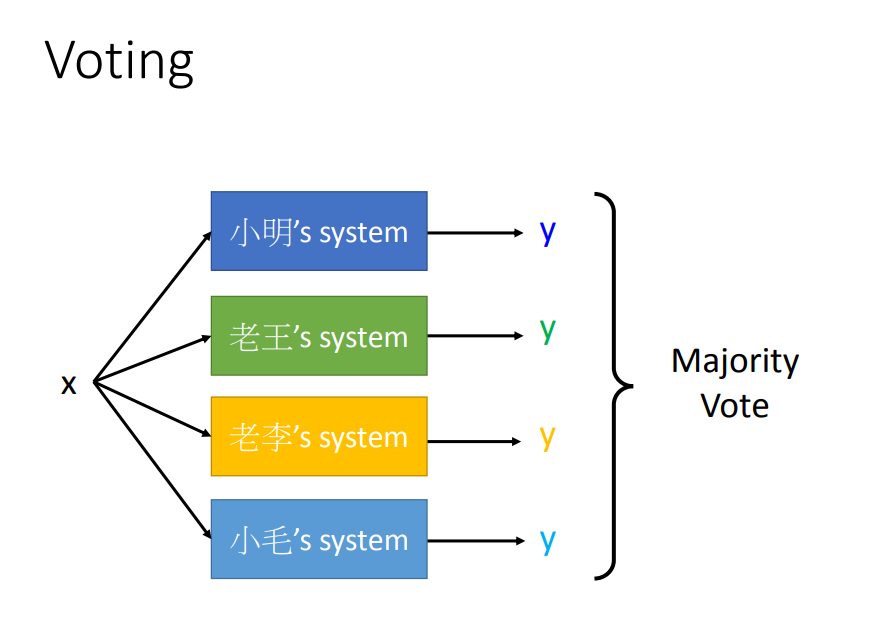
\includegraphics[scale=0.5]{Part1/Chapter/images/voting.png}}
    \caption{AdaBoost Experienment}
\end{figure}

\section{Stacking}
做Stacking时你要将training data分成两笔,一笔训练单模型一笔训练final classifier,目的是要避免过拟合的单模型获得大的权重。
\begin{figure}[H]
    \centerline{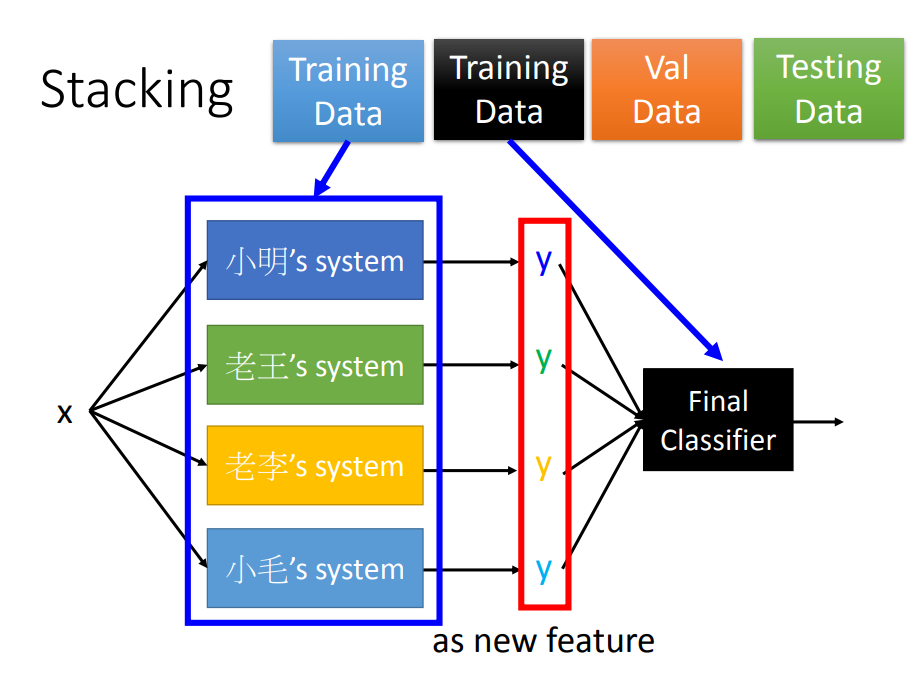
\includegraphics[scale=0.5]{Part1/Chapter/images/stacking.png}}
    \caption{AdaBoost Experienment}
\end{figure}
